\documentclass[letterpaper]{article}
\usepackage{aaai}
\usepackage{url}
\usepackage{fullpage}
\usepackage{graphicx,curves}
\usepackage{amsmath}
\usepackage{amssymb}
%\usepackage{cmbright}
\usepackage{latexsym}
\usepackage{multirow}
\usepackage[algoruled,vlined,linesnumbered]{algorithm2e}
\usepackage{wrapfig}
\usepackage{pdfsync}

\usepackage[bitstream-charter]{mathdesign}
%\renewcommand*\ttdefault{lmvtt}
\usepackage[T1]{fontenc}
\usepackage{natbib}

\newtheorem{df}{Definition}
\newtheorem{notation}{Notation}
\newtheorem{theorem}{Theorem}
\newtheorem{lemma}{Lemma}[section]
\newtheorem{col}{Corollary}

%\newcommand{\bt}{\begin{theorem}\em}
%\newcommand{\et}{\end{theorem}}
\newcommand{\Qed}{$\blacksquare$}
\newcommand{\qed}{$\Box$}
%\newcommand{\proof}{{\bf Proof. }}
\newcommand{\nin}{\noindent}
%\newcommand{\bea}{\begin{eqnarray}}
%\newcommand{\eea}{\end{eqnarray}}
%\newcommand{\bdf}{\begin{df}\em}
%\newcommand{\edf}{\end{df}}
%\newcommand{\ben}{\begin{enumerate}}
%\newcommand{\een}{\end{enumerate}}
\newcommand{\ie}{\item}
\newcommand{\dist}{\operatorname{dist}}
\newcommand{\avg}{\operatorname{avg}}

\newcommand{\citea}[1]{\citeauthor{#1} (\citeyear{#1})}

\numberwithin{equation}{section}
\numberwithin{theorem}{section}
\numberwithin{lemma}{section}
\numberwithin{df}{section}

\setcounter{secnumdepth}{3} %% this gives us back SECTION NUMBERS!

\graphicspath{ {./images/} }


\title{A Neural Network Case Base for Real-Time Searching}

\nocopyright

\author{Zeyi Wang \\
    Department of Computing Science \\ University of Alberta \\
    Edmonton, Alberta, T6G 2E8, Canada \\
    {\texttt{zeyi2@ualberta.ca} }}


\begin{document}

    \maketitle

    \textit{(When I use "I" instead of "we", that means that part is my personal reflections and will changed in the final report.)}

    \begin{abstract}
        % Introduce and motivate the problem. State the main idea of your solution approach and highlights of its evaluation.
        Some real-time search algorithms use a case base to store previously solved problems and use the case base to build a new solution for an unknown problem in the real-time.
        Larger case bases leads to better performance at the cost of slower query time.
        In this paper, we build a neural network that is trained on the cases and achieve
        constant time for queries in any size case bases.

    \end{abstract}


    \section{Introduction}\label{sec:introduction}

    % Informally introduce and motivate your problem here.

    Using a case base is common technique in real-time search algorithms.
    When an agent encounters a previously unknown task, it searches in its case base for similar situations, and infers a solution from the cases.
    As a case base covers more cases, an agent utilizing the case base will be more likely to find similar situations and solutions.
    However, the time cost of retrieving similar cases also goes up when the case base is larger.
    In this paper, we purpose Neural Network Case Base (NNCB), a case base that benefits from more cases, but does not suffer from the extra time cost.

    Right now I have a few ideas of doing this.
    \begin{itemize}
        \item build a data base for inferring amount of heuristic updates
        \item build a data base for inferring actions
        \item build a data base for inferring an optimal path
    \end{itemize}


    \section{Problem Formulation}\label{sec:problem-formulation}

    % Define the problem formally, including the performance criteria motivated by the introduction. The reader needs to know how to assess your approach's success or failure.

    We define a heuristic problem as a directed graph containing a finitely many number of \textit{states}, in which one is the \textit{start} and one is the \textit{goal}, and \textit{edges} connecting adjacent states with fixed costs of 1.
    The agent has a single \textit{current state} at every time step.
    The agent can take an action by following an edge to change its current state.
    The \textit{solution cost} is the sum of all edge costs of a path the agent can follow to go from the start state to the goal state.
    The algorithm has to be complete so it is comparable to the other algorithms.


    \section{Related Work}\label{sec:related-work}

    So far I have been comparing my algorithm with weighted LRTA* \citea{lrta} \citea{weighted_lrta}.
    I implemented the neural network using pytorch by \citea{pytorch}.
    One of the approaches I am going to try involve predicting the amount of learing and there's previous work on that by \citea{learning_cost}.
    I drew inspiration from \citea{dlrta} \citea{knnlrta} \citea{hcdps} for using a case base.
    I also drew inspiration from \citea{rtnn} on using a neural network on real-time search problems.


    \section{Proposed Approach}\label{sec:proposed-approach}

    % Describe your ideas for the proposed approach informally at first. Show how the proposed approach addresses the shortfalls of the related research that you discussed above. Then describe the approach formally and precisely enough to be reproduced by an independent researcher.
    For this midterm report, most of my effort has been coding infrastructures (e.g, map/scene parsing, map/scene/path/heuristic-updates visualizations, agent-map interaction framework).
    See Figure ~\ref{fig:lrta_path} and Figure ~\ref{fig:lrta_h} for visualizations.

    \begin{figure}[h]
        \caption {LRTA Planned Path Visualized}
        \centering
        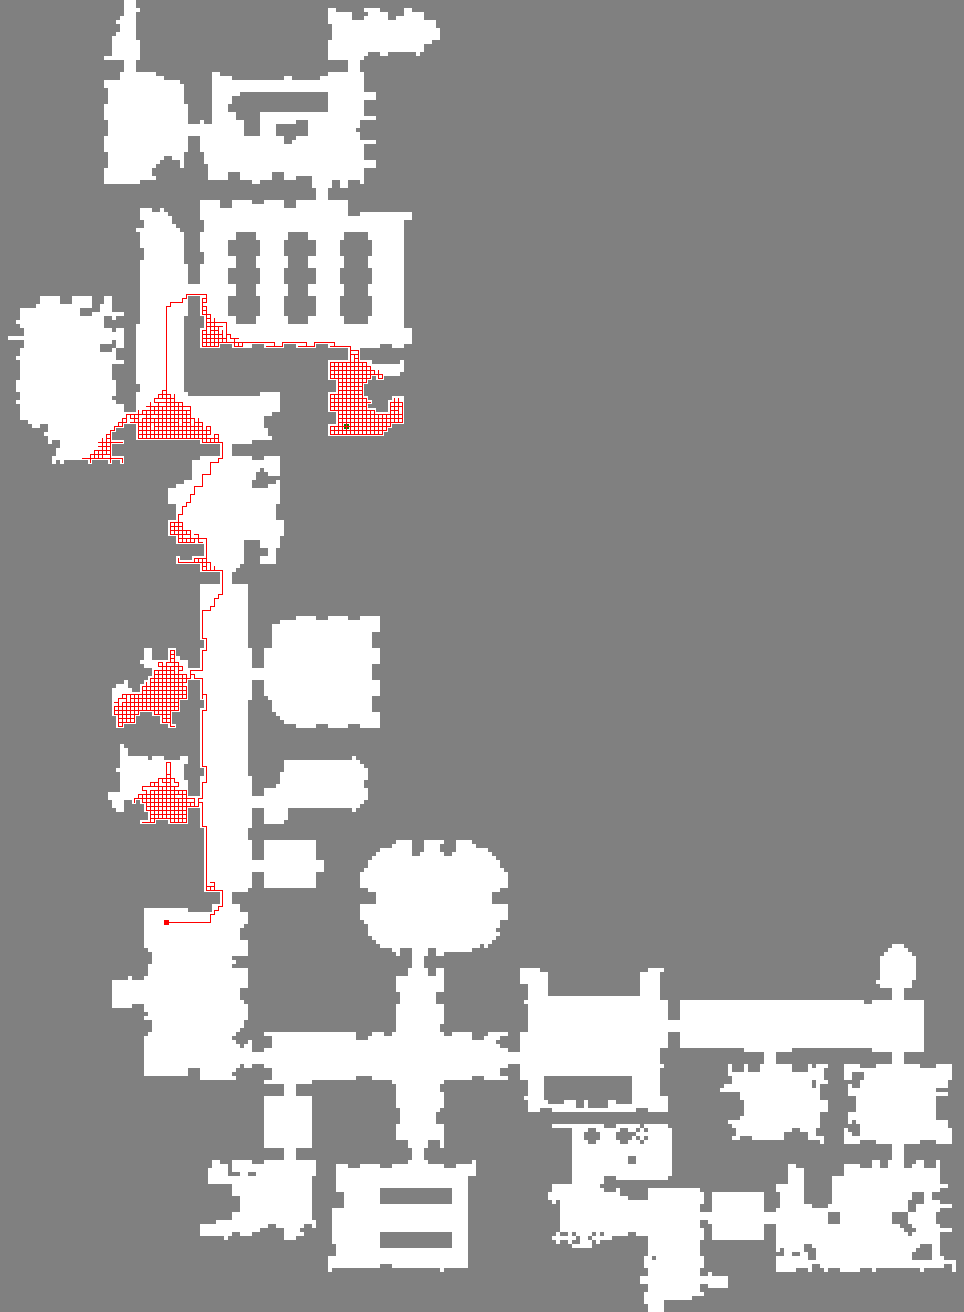
\includegraphics[width=0.5\textwidth]{lrta_path}
        \label{fig:lrta_path}
    \end{figure}

    \begin{figure}[h]
        \caption {LRTA Heuristic Updates Visualized}
        \centering
        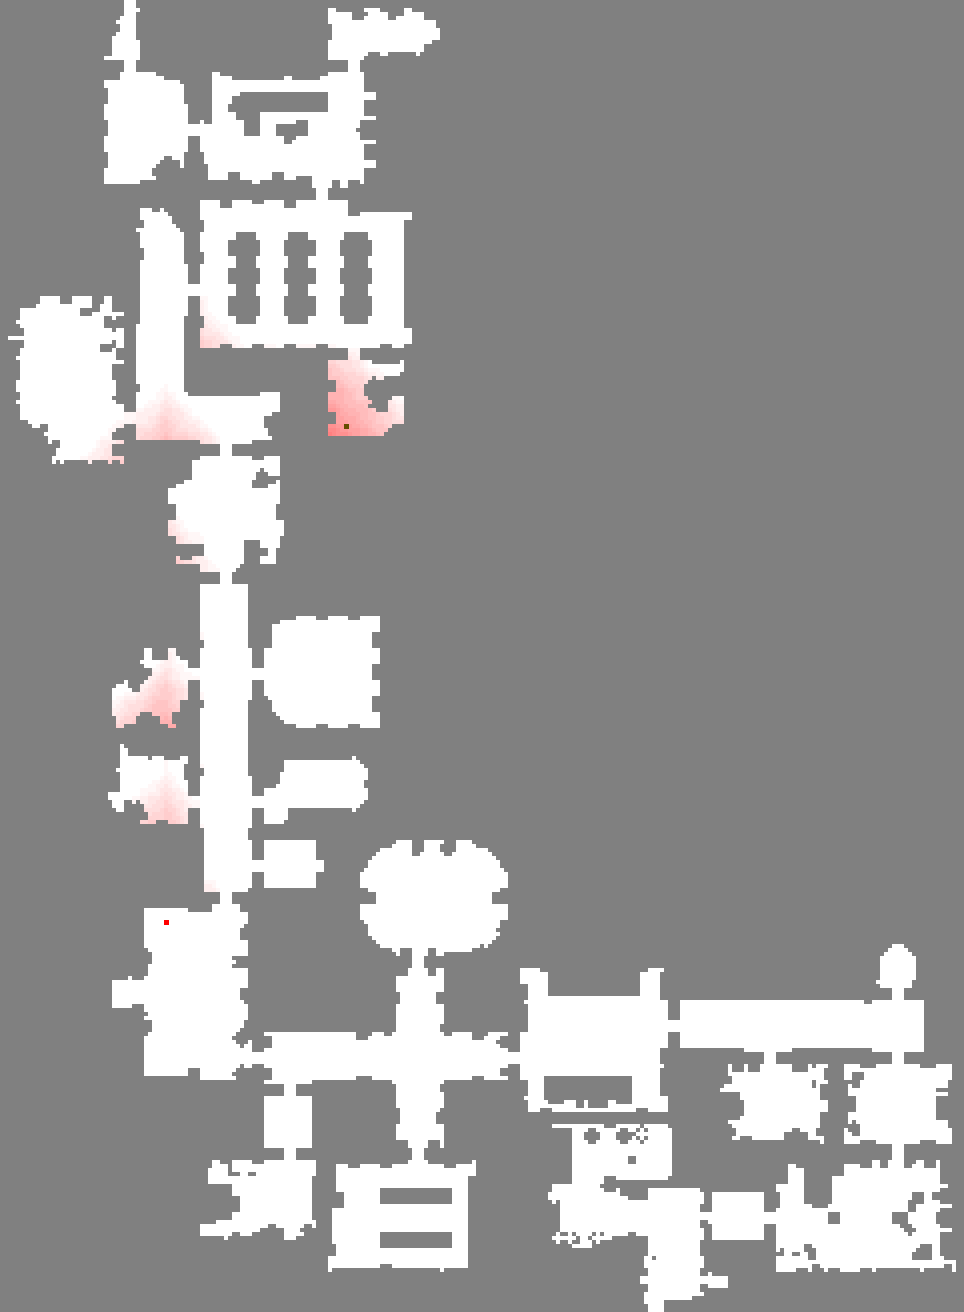
\includegraphics[width=0.5\textwidth]{lrta_h}
        \label{fig:lrta_h}
    \end{figure}

    The first thing I tried is to build a case base to predict heuristic updates from a view and its distance to the goal.

    Formally, for each entry in the case base, we have:
    \begin{itemize}
        \item $V_{i, j}$: a 7x7 matrix around the current state
        \item $d_{i, j}$: a 2D vector containing the difference between the goal and the current state
        \item $h_{i, j}$: the difference between the current state and the goal state
    \end{itemize}

    To use the case base, we start with a standard LRTA* procedure.
    When the agent wants to update a heuristic at given position $i, j$, instead of update the heuristic with a new $f$, the agent query the case base with $V_{i, j}$ and $d_{i, j}$.
    Right now my program does this by finding the nearest neighbors in the case base and averaging them.
    However, this part will be replace by a neural network later.

    (I also want to try predicting a move instead, we will see.)

    % If you decide to use pseudocode (e.g., Algorithm~\ref{alg:fAlg})\footnote{Reproduced with permission from work by~\citea{flow}.}, make sure you complement it with a plain English description. Additionally hand trace your pseudocode line by line (make sure you refer to the line numbers in your pseudo-code) on a simple example.

    % End this section formulating your hypothesis. For instance, ``my algorithm converges faster than X but uses more memory than Y under conditions A,B,C". Link your hypothesis to the motivation of the problem you gave earlier in the paper. For instance, if your hypothesis is about fast real-time operation then you should link it to the requirements of the problem at hand described earlier in the paper.


    \section{Theoretical Analysis}\label{sec:theoretical-analysis}

    % Discuss expected properties of your algorithm. For instance, what is the run-time complexity in time and space? Under what assumptions is your algorithm guaranteed to find a solution? If it is a learning algorithm, under which conditions will it converge?

    \subsection{Completeness}\label{subsec:completeness}
    We keep track of the number of visitations of each state.
    Once the number of visitation of a certain state exceeds $M$, a constant that we select, then the agent plan with vanilla LRTA* on that state.
    Since LRTA* is complete, and our algorithm at most plans $M * number of states$ times, the whole algorithm is complete.

    \subsection{Offline Time Complexity}\label{subsec:offline-time-complexity}
    The time is linear to the number of cases generated.

    \subsection{Offline Space Complexity}\label{subsec:offline-space-complexity}
    Since we are training a neural network with cases, we don't need to store the cases explicitly and the cases can be discarded once the network is trained.
    As a result, the offline space required by the algorithm is purely based on the number of parameters of the network, which is a constant.

    \subsection{Online Time Complexity}\label{subsec:online-complexity}
    Once we train a neural network for the case base, each query takes a fixed amount of computational time.
    Since the LRTA* backbone of the algorithm also runs in constant time, the whole algorithm runs in constant time.

    \subsection{Online Space Complexity}\label{subsec:online-space-complexity}
    The agent only store sub-goals in its memory and the number of sub-goals is upper-bounded by the number of states in the map.
    Hence, the online space complexity is a constant.


    \section{Empirical Evaluation}\label{sec:empirical-evaluation}

    % Support your hypothesis formulated above. First describe your empirical testbed in enough detail for an independent researcher to reproduce. Then describe all parameters of your algorithm as applied to the testbed. Finally present the results.

    % Do not be shy to list negative results as well --- they still improve our understanding of the field. Make sure your describe your experimental set up in enough detail for other researchers to replicate your work.

    % A solid empirical study not only offers some findings but also sheds light on how confident we should be about them. This can be accomplished through statistical tests (e.g., the T-test) and/or confidence intervals (e.g., Figure~\ref{fig:convPC}).

    Evaluate on \textit{Dragon Age: Origins} (DAO) maps provided by \citea{benchmarks}.
    So far I evaluated the draft version (not using a neural network) on one map and compared it with weight LRTA* ($w = 4$), and their suboptimality is roughly the same.
    I am planning to evaluate my algorithm on more DAO maps.
    In addition, I would like to split the pool of maps into a \textit{training pool} and a \textit{testing pool}.
    I will try to build the case base on the training pool and see if the algorithm works well on the testing pool.


    \section{Discussion}\label{sec:discussion}

    % Discuss your results with respect to the hypotheses you formulated and the demands of the problem at hand. Do not be shy to admit that you do not understand some of the results you obtained. Leave them as open questions for further research.

    We think using a neural network to build a case base is powerful idea and has a huge potential.
    We can discard the collected cases after the training is done (or even discard them as we train) to achieve a constant offline space complexity.
    We can also have constant time look up in the case base no matter how many cases we collected.
    We can think of a neural network to be the ultimate way to compress information in a case
    base to a fixed size.


    \section{Future Work}\label{sec:future-work}

    % Describe possible extensions (e.g., if you were to take on this project as your thesis work).

    One thing we would like to try is to create a neural network powered case base for querying optimal paths.
    The input of the network will be the start position and the goal position.
    The output of the network will be a sequence of hill-climbable sub-goals.
    Online, the agent retrieves the sub-goals and follows along by hill-climbing.
    Algorithms like kNN LRTA* suffers from case base offline space complexity and online time complexity.
    However, if we can train our case base with infinitely many cases without worrying about the consequences, we can make that infinite knowledge shines.


    \section{Conclusions}\label{sec:conclusions}

    % Refresh the reader on the problem at hand, motivation, shortfalls of the previous work, ideas of your new algorithm and the results of the empirical study. Briefly re-state the contributions your paper makes here.

    I expect to draw a conclusion base on my empirical evaluation.


    \section*{Acknowledgments}

    % Acknowledge any help you already received.
    I gratefully acknowledge the help by Vadim Bulitko, without which the present study could not have been completed.


    \bibliography{projectReport}
    \bibliographystyle{aaai}

\end{document}
